Im Folgenden sollen die beschriebenen Ergebnisse aus den vorherigen Abschnitten \ref{sec:ergebnisseSichtpruefungDurchLichtstreuung} und \ref{sec:ergebnisseDeflektometrischeRegistrierung} aufgegriffen und bewertet werden.
Das Ziel ist es abhängig vom Anwendungsfall ein passendes Verfahren vorzuschlagen und die Schwächen und Stärken der Verfahren anzusprechen.

\p
Für das Verfahren \glqq Sichtprüfung durch Lichtstreuung\grqq ~fällt im Abschnitt \ref{sec:ergebnisseSichtpruefungDurchLichtstreuung} auf, dass es sich besonders gut für die Durchlichtauswertung von transparenten Prüfobjekten eignet.
Es ist möglich bereits sehr kleine Defekte, wie z. B. sehr leichte Kratzer oder Laser-Gravuren auf den Objektoberflächen zu erkennen (siehe Abbildung \ref{tikz:abbErkennbareKleineDefekteLichtstreuung}).

% Abbildung: Erkennbare kleine Defekte
{
	\begin{figure}[H]
		\centering
		\begin{tikzpicture}[every node/.style={inner sep=0,outer sep=0}]

	\node [anchor=north east] (img1) at (-0.03\textwidth,0) {\includegraphics[width=.4\textwidth]{05_ergebnisse/ergDiskussion/figures/lasergravur}};
	\node [below=0.2cm of img1] {Ausschnitt von Brillenglas 1};
	\node [anchor=north west] (img2) at (0.03\textwidth,0) {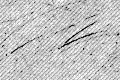
\includegraphics[width=.4\textwidth]{05_ergebnisse/ergDiskussion/figures/polierfehler}};
	\node [below=0.2cm of img2] {Ausschnitt von Brillenglas 2};
	
\end{tikzpicture}
\caption[Erkennbare kleine Defekte oder Laser-Gravur]{Erkennbare kleine Defekte oder Laser-Gravuren durch Durchlichtauswertung mit Verfahren \glqq Sichtprüfung durch Lichtstreuung\grqq ~(siehe Kapitel \ref{chp:sichtpruefungDurchLichtstreuung}) Linkes Teilbild: Erkennbare Lasergravur, Rechtes Teilbild: Leichte Kratzer durch Fehler bei der Polierung}
		\label{tikz:abbErkennbareKleineDefekteLichtstreuung}
	\end{figure}
}

\noindent
Außerdem ist es möglich für transparente Objekte durch die Durchlichtauswertung auch Defekte im Objekt, wie z. B. Lufteinschlüsse in Gläsern festzustellen.
Dies konnte allerdings nicht nachgeprüft werden, da solche Defekte in den zur Verfügung stehenden Prüfobjekten nicht vorhanden waren.

\p
Für nicht-transparente kann das Verfahren \glqq Sichtprüfung durch Lichtstreuung\grqq ~ebenfalls verwertbare Bilder erzeugen um Defekte zu detektieren, allerdings gibt es hierbei schon erste Probleme.
Eine große Schwäche des Verfahrens ist die Abhängigkeit von Oberflächenbeschriftungen oder -aufdrucken.
Da stets Grauwerte der Kamerabilder verknüpft werden beeinflussen unterschiedliche Farben auf der Oberfläche das Ergebnis (siehe Abbildung \ref{img:delleBeschriftung}).

% Abbildung: Beschriftung Delle
{
	\begin{figure}[H]
		\centering
		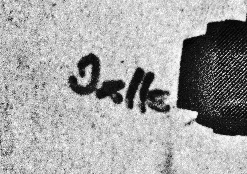
\includegraphics[width=0.4\textwidth]{05_ergebnisse/ergDiskussion/figures/delleBeschriftung}
		\caption[Sichtbare Beschriftung nach Anwendung des Verfahrens aus Kapitel \ref{chp:sichtpruefungDurchLichtstreuung}]{Sichtbare Beschriftung \glqq Delle\grqq ~nach Anwendung des Verfahren \glqq Sichtprüfung durch Lichtstreuung\grqq.}
		\label{img:delleBeschriftung}
	\end{figure}
}